%% Version 3/21/02

%%%%%%%%%%%%%%%%%%%%%%%%%%%%%%%%%%%%%%%%%%%%%%%%%%%%%%%%%%%%%%%%
%% Kluwer Proceedings Sample, ProcSamp.tex
%%
%% Kluwer Academic Press
%%
%% Prepared by Amy Hendrickson, TeXnology Inc., July 1999.
%%%%%%%%%%%%%%%%%%%%%%%%%%%%%%%%%%%%%%%%%%%%%%%%%%%%%%%%%%%%%%%%

%%%%%
%% LaTeX2e 
%% Uncomment documentclass, 
\documentclass{kapproc} % Computer Modern font calls

%% and, optionally, one or more 
%%   of the \usepackage commands below:

%%%%%
%% If you use a font encoding package, please enter it here, i.e.,
%  \usepackage{T1enc}

%%%%%
%  If you have MathTimes and MathTimesPlus fonts, you
%  may uncomment the line below and use them, but you are
%  not obligated to do so, and most authors do not have
%  these fonts. (You may need to edit m-times.sty to make the
%  font names match those on your system)

%  You must have the MathTimes fonts for this to work. They may be
%  purchased from the Y&Y company, http://www.YandY.com.

% \usepackage[mtbold,noTS1]{m-times}

%%%%%
% PostScript font calls
%
% If you use the procps PS font file, you may need to edit it
% to make sure the font names match those on your system. See
% the top of the procps.sty file for more info.

\usepackage{procps} 

%%%%%
% Style for inserting .eps files and rotating illustrations or tables

% possible options for graphicx:
% [dvips], [xdvi], [dvipdf], [dvipsone], [dviwindo], [emtex], [dviwin],
% [pctexps],  [pctexwin],  [pctexhp],  [pctex32], [truetex], [tcidvi],
% [oztex], [textures]

\usepackage{graphicx}
%\usepackage[dvipdf]{graphicx}

%%%%%%%%%%%%%%%%%%%%%
%% LaTeX209, 
%  Uncomment only one below, comment out similar commands above
%\documentstyle{kapproc} % Computer Modern fonts
%  \documentstyle[procps]{kapproc} %For PostScript fonts
%  (The m-times.sty works only with LaTeX2e)

%%%%%%%%%%%%%%%%%%%%%%%%%%%%%%%%%%%%%%%%%%%%%%%%%%%%%%%%%%%%%%%%%%%%%%%%%
%% Commands You Can Set or Change to Customize Your Book Format: ===>>>

% Running heads:
% ==============

%  Uncomment to make chapter title on left hand page
%  and section title on right hand page
%  \chapsectrunningheads


% Section heads:
% ==============

%%%
% \chaptersection % will use chapter.section form for section heads.

%%%
% Uncomment to make section heads appear in
%                    both upper and lower case.
\upperandlowercase

% \useuppercase % Uncomment to make section and subsection heads 
                %  appear in uppercase.

%%%
% How many levels of section head would you like numbered?
% 0= no section numbers, 1= section, 2= subsection, 3= subsubsection
\setcounter{secnumdepth}{2}

% Table of Contents:
% ==================
% How many levels of section head would you like to appear in the
%  Table of Contents?
%  0= chapter titles, 1= section titles, 2= subsection titles, 
%  3= subsubsection titles.
\setcounter{tocdepth}{2}

% Equation numbering:
% ===================

%%%
% \nochapequationnumber % will result in equation numbers that are (1)

%%%
% \sectionequationnumber % will result in equation numbers that are (1.1)
                         % and renumber for each section

% Default for kapproc is (equation number)

% Theorem numbering:
% ==================
% \nochaptheoremnumber % will make the theorem type environments number
       % only with the theorem number. 
       % Default is only theorem number for kapproc.

% Footnotes/Endnotes:
% ===================

% Default is endnotes that appear at the end of the chapter, above
% the references, or whereever \notes is written.

%%%
% To change footnotes to appear at bottom of page uncomment:
% \let\footnote\savefootnote

%%%
% Uncomment if you want footnotetext to appear at the bottom of the page:
%\let\footnotetext\savefootnotetext

%%%
% Uncomment if you want a ruled line above the footnote.
%\let\footnoterule\savefootnoterule

% Bibliography Style Settings:
% ============================
% Choose either kluwerbib or normallatexbib:

%%%
%\kluwerbib % will produce this kind of bibliography entry:

%  Anderson, Terry L.,...
%    continuing bib entry here

%  \cite{xxx} will print without brackets around the citation.
% \bibliographystyle{kapalike} % should be used when you use \verb+\kluwerbib+.

%%%
\normallatexbib %will produce bibliography entries as shown in the
                % LaTeX book

% [1] Anderson, Terry L.,
%     continuing bib entry

% \cite{xxx} will print with square brackets around the citation, i.e., [1].

% Any \verb+\bibliographystyle{}+ may be used with \verb+\normallatexbib+, but
% you should check with your editor to find the style preferred for
% your book.

% Change Brackets around Citation:
% ================================

%% Default with \kluwerbib is no brackets around citation. 
%% Default with \normallatexbib is square brackets around citation. 

% For parens around citation uncomment these:

%\let\lcitebracket(
%\let\rcitebracket)

% For square brackets around citation uncomment these:

%\let\lcitebracket[
%\let\rcitebracket]

% Draft Line:
% ===========
%  Optional, uncomment to make current time and `draft' appear at
%  bottom of page.

% \draft

%%%% <<== End Formatting Commands You Can Set or Change %%%%%%%%%%%%%%%%%
%%%%%%%%%%%%%%%%%%%%%%%%%%%%%%%%%%%%%%%%%%%%%%%%%%%%%%%%%%%%%%%%%%%%%%%%%

\begin{document}

%------------ article title  ------------------->>

% If you use \\'s , please supply an alternate version of the title
% in square brackets, i.e., 
%\articletitle[Communism, Sparta, and Plato]
%{COMMUNISM, SPARTA,\\ and PLATO}

\articletitle[MADES R1.0, user manual]{MADES R1.0,\\ user manual}

%% optional, to supply a shorter version of the title for the running head:
%%\chaptitlerunninghead{}

%\author{Baresi Luciano\\
%Bonvini Marco\\
%Ferretti Gianni\\
%Leva Alberto\\
%Rossi Matteo\\
%Sama Michele}

%% multiple authors may be separated with \\
%% \author{Samuel Bostaph\\
%% and Gregor Kariotis}

%------ author/affiliation choices -------------->>

%% Single author

% \author{}
% \affil{}
% \email{}

%% Multiple authors, single affiliation

% \author{Samuel Bostaph}
% \author{George Lewis}
% \and   % <=== Type in \and before the last author so that `and' will
% \author{Cleon Jones}    % print between the last two authors
                           % in the table of contents.

% \affil{}

%% Multiple authors, multiple affiliations

% First method:
--------------

\author{Baresi Luciano}
\affil{Politecnico di Milano}
\email{baresi@elet.polimi.it}
\author{Bonvini Marco}
\affil{Politecnico di Milano}
\email{bonvini@elet.polimi.it}
\author{Ferretti Gianni}
\affil{Politecnico di Milano}
\email{ferretti@elet.polimi.it}
\author{Leva Alberto}
\affil{Politecnico di Milano}
\email{leva@elet.polimi.it}
\author{Rossi Matteo}
\affil{Politecnico di Milano}
\email{rossi@elet.polimi.it}
\author{Sama Michele}
\affil{PuzzleDev s.n.c.}
\email{m.sama@puzzledev.com}


%------ prologue, abstract, keywords ----------->>
% optional prologue
%\prologue{<text>}{<author, year>}

\pagebreak 
% optional abstract
\begin{abstract}
MADES is a co-simulation tool aiming to generate feasible execution traces
for systems composed by a software component and an physical external device described in terms of its mechanical, electrical, and thermochemical 
properties which represent the environment in which the software component is running. The software component is simulated with a discrete time step representing the sampling time of sensors,
while its environment is simulated with a continuous time
representing the physical reaction of the system. The generated trace is deterministic for the environment, and non-deterministic for the software,
since it may include human interactions. In this document we give a general overview of MADES and of its components and we explain in details how it can be used to generate co-simulated traces.
\end{abstract}

% optional keywords
\begin{keywords}
MADES, ZOT, Modelica, trace generation, co-simulation
\end{keywords}


%------------ body of article ------------------->>
\pagebreak 
\section{General Overview}
\label{section:general-overview}

MADES is an open source co-simulation tool aiming to generate realistic execution traces for software components driving external devices inside a physical environment. The goal of MADES is to co-simulate both the software and the environment simultaneously and consistently.  This is done by means of a set of shared timed variables. The system declares a set of output
variables which are used as input for the environment. Similarly the environment declares a set of output variable which are given in input to the system. 

The co-simulation simulates the system with a discrete time, which 
represents the software response time. We call that delta time a 
simulation \emph{step}. Each step represent the time between the current 
co-simulation time and the following time plus $\delta$, where $\delta$ is 
the constant time duration of each steps. At each step
of the co-simulation the environment is simulated with a continuous 
time starting from the current time $t$ until $t +\delta$. 

After each step all the shared timed variables are flagged with
both the continuous time $t + \delta$ and the discrete time $s$ represented 
by the number of steps. For instance at the third step of co-simulation all the produced variables are flagged with $t = 3*\delta$ and $s = 3$.

The trace produced by MADES at the end of the co-simulation is the ordered 
set of all the shared variables from the beginning till the end of the co-simulation. Such trace is saved as in a file called \emph{madesOutput.xml} placed in the same folder of the simulated model.

\subsection{Simulators}

MADES uses an open architecture which allows developers to use their own
simulators during the co-simulation. At the moment the binding is static
and simulators are specified at runtime, however in the future a plug-in based architecture will be implemented allowing dynamic selection of the various
simulators.

The current version uses the temporal-logic solver ZOT~\cite{zotSolver} and 
the sat solver z3~\cite{z3SatSolver} to simulate the system and uses the Open Modelica Compiler (omc) for the environment~\cite{Fritzson05theopenmodelica}.

The co-simulations requires in input a ZOT and a Modelica models which will be instrumented and executed by MADES. For more informations about the input files see Section~\ref{section:input-models}. For information about how the model are instrumented see Section~\ref{section:models-instrumentation}. For technical
details in how to use a different simulator please see Section~\ref{section:expanding-mades}

\subsection{Downloading And Running MADES}

There are to ways to download MADES. Developers willing to extend the 
co-simulator can download the latest 
source of MADES from the repository on Google code~\cite{MadesSvn}. 
Users willing to simply run a co-simulation can download a re-distributable
package of MADES from the download section of the Google code MADES 
website.

MADES is entirely written in java 1.6 and therefore it requires the JRE to be installed. During our development we used the OpenSDK 1.6 and that is the evironment that we recommend.
In order for MADES to run correctly there are several dependencies which have to
be satisfied. MADES is supposed to be executed in a linux-like environment. 
The suggested environment is Ubuntu $11.04$. 
In addition MADES requires gcc, omc
and the list interpreter sbcl to be installed. Note that the Open Modelica Compiler must be of a version equals or newer than 1.7.0 (r9303). In addition ZOT and z3 to be installed
and available to the current user. For convenience we included the version 
of ZOT that we used during the development in the download 
section. For licenses issues we could not include z3,  however 
it is also available for free download~\cite{z3Website}

To facilitate the users we provide a bash install script which will automatically download and install all the required libraries. The install script is also available from the download page in the MADES Google code website.
Once MADES is currently installed it can be execute in two ways, as a shell 
command or with a GUI.

\subsection{Running MADES with the GUI}

Users willing to use MADES stand-alone should use the gui version. To do so the can simply double click on the \emph{Mades.jar} file and it should run. Alternatively the MADES' main form can be opened by running:\\
\begin{verbatim}
java -jar Mades.jar
\end{verbatim}

The GUI mode is the default mode to use MADES. Please note that if the GUI is invoked from a shell it will display in output all the log messages. Users having problems while simulating a particular model may find this output information very useful.

\begin{figure}[h]
	 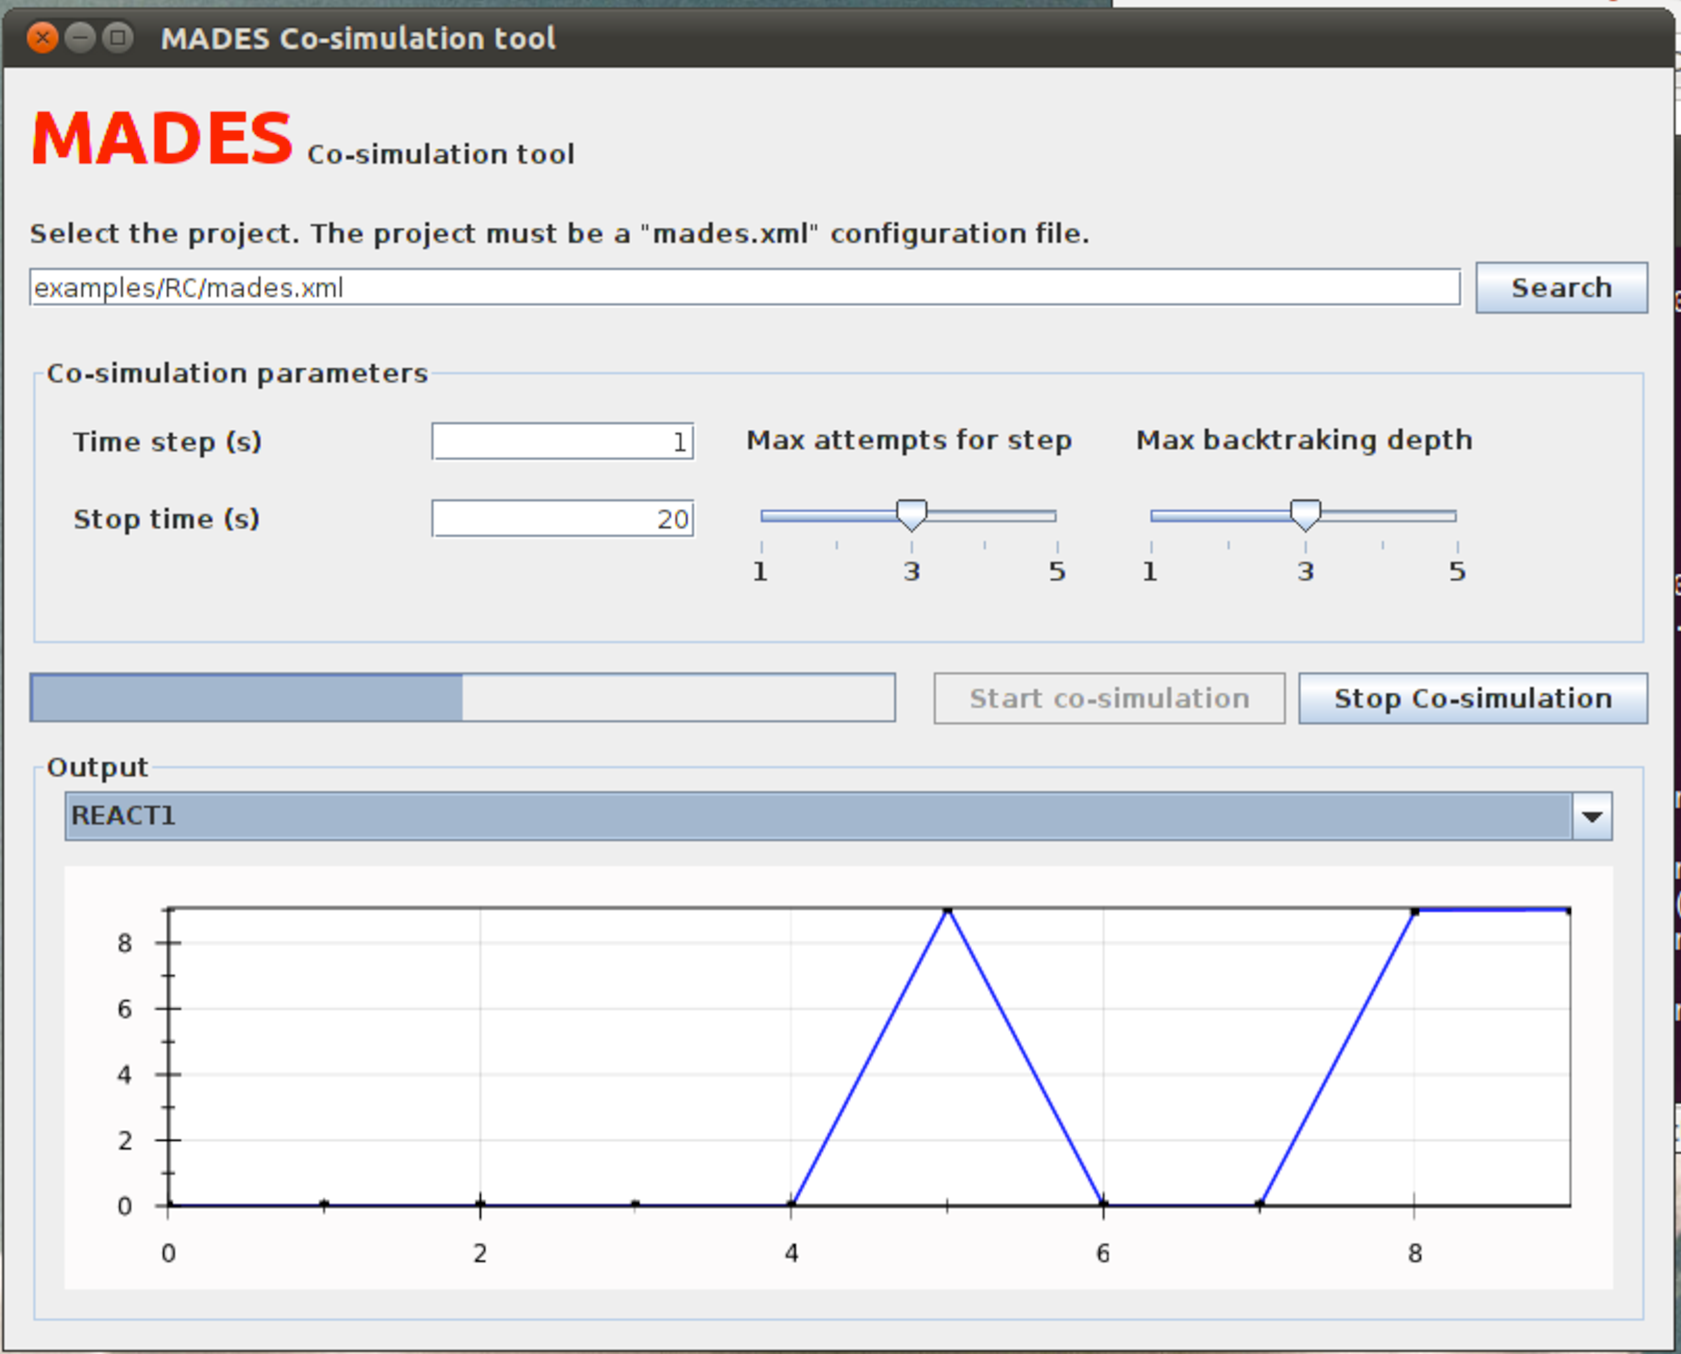
\includegraphics[width=12cm]{img/Mades-gui.pdf}
	 \caption{The MADES main GUI}
	 \label{fig:mades-gui}
\end{figure}

Figure~\ref{fig:mades-gui} shows the main window of the MADES GUI. To run a simulation the user must first select a \emph{mades.xml} file then press the start button. It is possible to specify different simulation parameters by changing the values on the main window.

At the bottom of the main window all the shared variables are plotted. Users may interactively zoom in and out as they please. They may also print or export the picture as PNG files.

\subsection{Running MADES From The Command Linel}

Users willing to run MADES as a shell command should run:\\
\begin{verbatim}
java -classpath ./:./Mades.jar mades.cosimulation.Cosimulator <model-name>
\end{verbatim}

If we execute the previous command without any parameter MADES terminates with the following error:\\
\begin{verbatim}
Cosimulator
ERROR: filename string not specified.
Usage: Mades <filename> 
             [-timeStep=1] 
             [-stopTime=20] 
             [-attemptsInStep=3] 
             [-backtrakingDepth=3]
\end{verbatim}
In order to work from command line MADES must be invoked specifying a \emph{mades.xml} file and all the required configuration parameters.

\section{Input Models}
\label{section:input-models}

To work properly MADES expects to find two set of files: the input models, which are specified by the user at runtime and a set of files used to instrument the given model as required by the co-simulator. Table~\ref{table:input-files} list the ones of which users should be aware of. All the other files are either generated during the compilation or created at runtime as results of the computation.

\begin{table}[h]
\caption{Mades input file}
\label{table:input-files}
\centering
\begin{tabular}{ l | l }
\sphline
File name &Description\\
\sphline
\sphline
mades.xml&The MADES configuration file\\
\sphline
zot/run.zot&The runner for the ZOT model\\
\sphline
zot/MODEL\_system.zot&The system model for ZOT\\
\sphline
zot/MODEL\_constraints&The system constraints for ZOT\\
\sphline
zot/MODEL\_history.zot&The system constraints created by the co-simulator during the execution\\
\sphline
modelica/sources/MODEL.mo&The source file of the environment model for Modelica\\
\sphline
modelica/MODEL&The instrumented and compiled model for Modelica\\
\sphline
modelica/MODEL\_init.xml&The initial parameters for Modelica\\
\sphline
modelica/MODEL\_res.csv&The simulation results generated by Modelica at each step\\
\sphline
madesOutput.xml&The trace file generated at the end of the cosimulation\\
\sphline
\end{tabular}
\end{table}

The file \emph{mades.xml} contains a description of how the system and the 
environment interacts.  All the shared variables must be defined here. If necessary also private variables belonging to the system or to the environment can be declared here. For convenience we declared here also ZOT private variables.

In addition to variable definition the xml file contains \emph{trigger groups} and \emph{trigger} definitions. A trigger represent a variable being monitored. Monitored variables are associated to a threshold value and with a boolean signal.
When the monitored variable has a value lower than the threshold their associated signals has value $0$. Contrarily when the variable is higher than the threshold its associated signal has value $1$.

Variables are monitored both to have trigger signals and to assure that they do not change their value more often than $\delta$. 
Each time a monitored variable changes their value Modelica trace them and invalidates the last step of the simulation.

If a trigger group contains more than a variable not only the single variables must
not cross their associated threshold more often than $\delta$ but also when one changes either the other change values simultaneously or the should not change sooner than $\delta$.

\section{Models Instrumentation}
\label{section:models-instrumentation}

The MADES co-simulator instruments the given models with additional
instructions required to ensure the correctness of the generated trace. The instrumentation depends on the simulation tools used.

The ZOT model is instrumented in order to keep trace of the previously simulated 
steps. The file \emph{run.zot} is added to the system model and instrumented in order to run the given model with an history extracted from the trace generated so far. In addition whenever a simulated step is rejected or when the co-simulator 
backtrack a previously accepted step its configuration is added to the history
as a configuration to be avoided.

The Modelica model is instrumented by adding trigger signals for the monitored variables and to invoke a print function every time a threshold is crossed. It is then recompiled before simulating the first step. By design the Modelica model is initialized with a set of initialization parameters located in the file
\emph{MODEL\_init.xml}. At each simulation step this file is instrumented with values resulting from the previous simulation steps. Similarly Modelica produces a
result file called \emph{MODEL\_res.csv} which contains all the simulated values. The co-simulator reads the output values at time $t + \delta$ and updates the values in the \emph{MODEL\_init.xml} file.

\section{How the Co-simulation Works}

The co-simulator starts from a given initial state and performs the simulation of both environment and system. At each step, starting from the configuration of the previous step, first the environment is simulated then the system is simulated using an intermediate configuration representing the system configuration at time $t$ and the system variables at time $t + \delta$. The result produced by this co-simulation
are correct under the assumption that all the shared variables keep their value for the whole step and that they change only at the end of each step.

Since the environmental variables simulated by Modelica are continuous and since they may change their value at any time the component wrapping Modelica must guarantee that they do not \emph{change} too quickly, where changing means to cross a threshold line. This is done by means of signals and signal groups. Internally the Modelica wrapper informs the co-simulator
if one of the signals or one of the signal groups has changed sign within a time shorter than $\delta$. When that happens the co-simulator rejects the simulation step and rolls back to the previous accepted environment simulation.  
Similarly Zot may fail to find a suitable solution if the given configuration is not satisfiable. Also in that case the the co-simulation rolls back.

Please note that since Modelica is deterministic repeating the same simulation twice will produce the same output. Once a not satisfying configuration has been reached the co-simulator needs to roll back not only Modelica but also the latest step simulated by Zot. In order to prevent Zot from re-simulating the same trace the co-simulator add the rejected step in the history of the Zot model as a configuration to avoid.

If after a certain number of attempts no valid configuration is generated the co-simulator rolls back to a previous step, then try again. This continues until the maximum backtrack limit is hit. If the limit is reached then the co-simulation fails. 

\section{Expanding MADES}
\label{section:expanding-mades}

MADES is structured as a set of pluggable components which can 
be replaced at compile time. Future versions of MADES will allow developers
to select which simulator to use at runtime.

The co-simulator invokes the system by calling a component implementing the interface \emph{SystemConnector}. Similarly the environment is accessed by invoking a class implementing
\emph{EnvironmentConnector}. Internally those components wraps a simulator and
invoke it as needed. The configuration resulting from each simulation step is stored using the Memento design pattern. Instances of the class \emph{SystemMemento} store the system configuration while instances of \emph{EnvironmentMemento} stores the environment state. 

Developers willing to connect a third party simulator to modelica should implement a wrapper implementing the opportune connector interface and should return an instance of the right memento at each invocation.


%------------ end of article ------------------->>

%% optional
%\section{Summary}

%% optional
%\begin{acknowledgments}
%...
%\end{acknowledgments}


%% appendix optional
%\appendix{This is the Appendix Title}
%This is an appendix with a title.

%\appendix{}
%This is an appendix without a title.

%
% Bibliography made with BibTeX:
\bibliographystyle{kapalike}
\chapbblname{Mades}
\chapbibliography{Mades}

\end{document}

Other commands, and notes on usage:

-----
Possible section head levels:
\section{Introduction}
\subsection{This is subsection}
\subsubsection{This is subsubsection}
\paragraph{This is the paragraph}

-----
Captions:
 If you use index commands within a caption, precede \inx or \inxx with
 \protect.

\begin{figure}[h]
\caption{\protect\inx{Oscillograph} for memory address access ....
memory plane.}
\end{figure}

-----
Tables:
 Remember to use \centering for a small table and to start the table
 with \hline, use \hline underneath the column headers and at the end of 
 the table. Column headers should be in italic:

\begin{table}[h]
\caption{Small Table}
\centering
\begin{tabular}{ccc}
\sphline
\it one&\it two&\it three\\
\sphline
C&D&E\\
\sphline
\end{tabular}
\end{table}

For a table that expands to the width of the page, write

\begin{table}
\begin{tabular*}{\textwidth}{@{\extracolsep{\fill}}lcc}
\hline
....
\end{tabular*}
%% Sample table notes:
\begin{tablenotes}
$^a$Refs.~19 and 20.

$^b\kappa, \lambda>1$.
\end{tablenotes}
\end{table}

-----
%% Use \printindex if you are using the LaTeX Makeindex commands:
%% \makeindex and \index{}
%\printindex

%% Use \kluwerprintindex if you are using the Kluwer indexing macros:
%%(\inx{} and \inxx{})
\kluwerprintindex

Kluwer Index commands:
\inx{term} will print `term' in text but will also send `term' and its
page number to the .inx file.

\inxx{term} will not print in text but will send term and its page number to
the .inx file.

\inxx{term,second term} will not print in text but will send `second term'
to inx file to print underneath `term' in the index.

1) Run Latex on file,
2) Run sort routine on file ie. `sort < filename.inx > filename.srt' on
your system to produce a filename.srt file
3)\printindex at end of book will input filename.srt and print index.

See documentation for more information.

-----
Algorithm.
Maintains same fonts as text (as opposed to verbatim which uses fixed
width fonts). Space at beginning of line will be maintained if you
use \ at beginning of line.

\begin{algorithm}
{\bf state\_transition algorithm} $\{$
\        for each neuron $j\in\{0,1,\ldots,M-1\}$
\        $\{$   
\            calculate the weighted sum $S_j$ using Eq. (6);
\            if ($S_j>t_j$)
\                    $\{$turn ON neuron; $Y_1=+1\}$   
\            else if ($S_j<t_j$)
\                    $\{$turn OFF neuron; $Y_1=-1\}$   
\            else
\                    $\{$no change in neuron state; $y_j$ remains %
unchanged;$\}$ .
\        $\}$   
$\}$   
\end{algorithm}

-----
Sample quote:
\begin{quote}
quotation...
\end{quote}

-----
Listing samples

\begin{enumerate}
\item
This is the first item in the numbered list.

\item
This is the second item in the numbered list.
\end{enumerate}

\begin{itemize}
\item
This is the first item in the itemized list.

\item
This is the first item in the itemized list.
This is the first item in the itemized list.
This is the first item in the itemized list.
\end{itemize}

\begin{itemize}
\item[]
This is the first item in the itemized list.

\item[]
This is the first item in the itemized list.
This is the first item in the itemized list.
This is the first item in the itemized list.
\end{itemize}

----
Glossary:

\begin{glossary}
\term{xxx}Text...
\term{yyy}Text...
\end{glossary}

i.e.,
\begin{glossary}
\term{GaAs}Gallium Arsinide. For similar device sizes GaAs transistors 
have three to
five times greater transconductance than those of of silicon bipolar
and MOS transistors.

\term{VLSI}Very Large Scale Integration. Since the mid-1970's 
VLSI technology has been successfully used in many areas, but its effect on
computers of all shapes and sizes has been the most dramatic. Some of the
application areas got boosts in performance while others became
feasible.

\end{glossary}







